
 Consider the figure below:
\begin{center}
 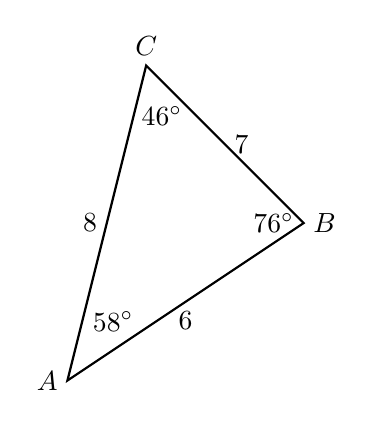
\begin{tikzpicture}
 
 \draw (0,0) --(3,2)--(1,4)--cycle  [thick,-,>=latex];

  \draw node[left] at (0,0) {$A$};
  \draw node[right] at (3,2) {$B$};
      \draw node[above] at (1,4) {$C$};

 \draw node[below] at (1.5,1) {$6$};
 \draw node[right] at (2,3) {$7$};
 \draw node[left] at (.5,2) {$8$};
   
 \draw node[right] at (.2,.75) {$58^\circ$};
  \draw node[left] at (3,2) {$76^\circ$};
      \draw node[below] at (1.2,3.6) {$46^\circ$};


\end{tikzpicture}
\end{center}


Which equation holds true?

(Note: For any triangle with sides $a,b,c$ that are opposite angles $A,B,C$ respectively, $\frac{\sin(A)}{a}=\frac{\sin(B)}{b}=\frac{\sin(C)}{c}.$)


\ifsat
	\begin{enumerate}[label=\Alph*)]
		\item    $\frac{\sin(58^\circ)}{8}=\frac{\sin(76^\circ)}{7}$
		\item  $\frac{\sin(76^\circ)}{8}=\frac{\sin(58^\circ)}{7}$ %
		\item $\frac{\sin(46^\circ)}{6}=\frac{\sin(58^\circ)}{8}$
		\item  $\frac{\sin(76^\circ)}{8}=\frac{\sin(46^\circ)}{8}$
	\end{enumerate}
\else
\fi

\ifacteven
	\begin{enumerate}[label=\textbf{\Alph*.},itemsep=\fill,align=left]
		\setcounter{enumii}{5}
		\item    $\frac{\sin(58^\circ)}{8}=\frac{\sin(76^\circ)}{7}$
		\item  $\frac{\sin(76^\circ)}{8}=\frac{\sin(58^\circ)}{7}$ %
		\item $\frac{\sin(46^\circ)}{6}=\frac{\sin(58^\circ)}{8}$
		\addtocounter{enumii}{1}
		\item $\frac{\sin(58^\circ)}{6}=\frac{\sin(76^\circ)}{8}$
		\item  $\frac{\sin(76^\circ)}{8}=\frac{\sin(46^\circ)}{8}$
	\end{enumerate}
\else
\fi

\ifactodd
	\begin{enumerate}[label=\textbf{\Alph*.},itemsep=\fill,align=left]
		\item    $\frac{\sin(58^\circ)}{8}=\frac{\sin(76^\circ)}{7}$
		\item  $\frac{\sin(76^\circ)}{8}=\frac{\sin(58^\circ)}{7}$ %
		\item $\frac{\sin(46^\circ)}{6}=\frac{\sin(58^\circ)}{8}$
		\item $\frac{\sin(58^\circ)}{6}=\frac{\sin(76^\circ)}{8}$
		\item  $\frac{\sin(76^\circ)}{8}=\frac{\sin(46^\circ)}{8}$
	\end{enumerate}
\else
\fi

\ifgridin
  $\frac{\sin(76^\circ)}{8}=\frac{\sin(58^\circ)}{7}$ %
		
\else
\fi

